\documentclass{article}
\usepackage{tikz}
%%%<
\usepackage{verbatim}
\usepackage[active,tightpage]{preview}
\PreviewEnvironment{tikzpicture}
\setlength\PreviewBorder{5pt}%
%%%>
\usetikzlibrary{arrows}
\begin{document}
\begin{tikzpicture}[->,>=stealth',shorten >=1pt,auto,node distance=3cm,
  thick,main node/.style={circle,draw,font=\sffamily\Large\bfseries}]


\setlength\fboxsep{0pt}
\setlength\fboxrule{1pt}

    \node (downxn) [label=above:$x_n$,label=right:render] {$\Bigg\Downarrow$};
    \node (im1a) [below of=downxn]{\fbox{
\includegraphics[scale=0.5]{whisker1}}};
    \node (downim1a) [below of=im1a,label=right:$\phi$-transform] {$\Bigg\Downarrow$};
    \node (im2a) [below of=downim1a]{\fbox{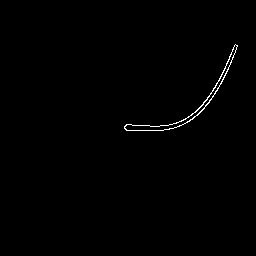
\includegraphics[scale=0.5]{whisker1_canny}}};

    \node (compare) [right of=im2a,label=below:compare]{$\longleftrightarrow$};
    \node (im2b) [right of=compare]{\fbox{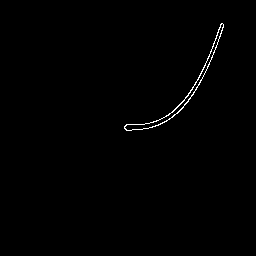
\includegraphics[scale=0.5]{whisker2_canny}}};
    \node (downim1b) [above of=im2b,label=right:$\phi$-transform] {$\Bigg\Downarrow$};
    \node (im1b) [above of=downim1b]{\fbox{
\includegraphics[scale=0.5]{whisker2}}};
    \node (downreal) [above of=im1b,label=right:pre-processing,label=above:$I_n$] {$\Bigg\Downarrow$};

    \node (resultarrow) [right of=im2b]{$\Longrightarrow$};
    \node (result) [right
    of=resultarrow]{\fbox{
\includegraphics[scale=0.5]{whisker_compare_canny}}};

\end{tikzpicture}
\end{document}


